\documentclass[12pt]{beamer}
\newenvironment{ConCodigo}[1]
  {\begin{frame}[fragile,environment=ConCodigo]{#1}}
  {\end{frame}}
\graphicspath{{Imagenes/}{../Imagenes/}}
\usepackage[utf8]{inputenc}
\usepackage[spanish]{babel}
\usepackage{hyperref}
\usepackage{etex}
\reserveinserts{28}
\usepackage{amsmath}
\usepackage{amsthm}
\usepackage{mathtools}
\usepackage{multicol}
\usepackage{multirow}
\usepackage{tabulary}
%\usepackage{tabularx}
\usepackage{booktabs}
\usepackage{nccmath}
\usepackage{biblatex}
\usepackage{epstopdf}
\usepackage{graphicx}
\usepackage{siunitx}
\sisetup{scientific-notation=true}
%\usepackage{fontspec}
\usepackage{lmodern}
\usepackage{float}
\usepackage[format=hang, font=footnotesize, labelformat=parens]{caption}
\usepackage[autostyle,spanish=mexican]{csquotes}
\usepackage{standalone}
\usepackage{tikz}
\usepackage[siunitx]{circuitikz}
\usetikzlibrary{arrows,patterns,shapes}
\usetikzlibrary{decorations.markings}
\usetikzlibrary{arrows}
\usepackage{color}
%\usepackage{beton}
%\usepackage{euler}
%\usepackage[T1]{fontenc}
\usepackage[sfdefault]{roboto}  %% Option 'sfdefault' only if the base font of the document is to be sans serif
\usepackage[T1]{fontenc}
\renewcommand*\familydefault{\sfdefault}
\DeclareGraphicsExtensions{.pdf,.png,.jpg}
\usepackage{hyperref}
\renewcommand {\arraystretch}{1.5}
\newcommand{\python}{\texttt{python}}
\usefonttheme[onlymath]{serif}
\setbeamertemplate{navigation symbols}{}
\usetikzlibrary{patterns}
\usetikzlibrary{decorations.markings}
\tikzstyle{every picture}+=[remember picture,baseline]
%\tikzstyle{every node}+=[inner sep=0pt,anchor=base,
%minimum width=2.2cm,align=center,text depth=.15ex,outer sep=1.5pt]
%\tikzstyle{every path}+=[thick, rounded corners]
\setbeamertemplate{caption}[numbered]
\newcommand{\ptm}{\fontfamily{ptm}\selectfont}
%Se usa la plantilla Warsaw modificada con spruce
\mode<presentation>
{
  \usetheme{Warsaw}
  \setbeamertemplate{headline}{}
  \useoutertheme{default}
  \usecolortheme{beaver}
  \setbeamercovered{invisible}
}
\AtBeginSection[]
{
\begin{frame}<beamer>{Contenido}
\normalfont\mdseries
\tableofcontents[currentsection]
\end{frame}
}

\usepackage{listings}
\lstset{ %
language=Python,                % choose the language of the code
basicstyle=\small,       % the size of the fonts that are used for the code
numbers=left,                   % where to put the line-numbers
numberstyle=\small,      % the size of the fonts that are used for the line-numbers
stepnumber=1,                   % the step between two line-numbers. If it is 1 each line will be numbered
numbersep=5pt,                  % how far the line-numbers are from the code
backgroundcolor=\color{white},  % choose the background color. You must add \usepackage{color}
showspaces=false,               % show spaces adding particular underscores
showstringspaces=false,         % underline spaces within strings
showtabs=false,                 % show tabs within strings adding particular underscores
frame=single,   		% adds a frame around the code
tabsize=2,  		% sets default tabsize to 2 spaces
captionpos=b,   		% sets the caption-position to bottom
breaklines=true,    	% sets automatic line breaking
breakatwhitespace=false,    % sets if automatic breaks should only happen at whitespace
escapeinside={\%},          % if you want to add a comment within your code
stringstyle =\color{magenta},
keywordstyle = \color{blue},
commentstyle = \color{green},
identifierstyle = \color{red}
}
\title{Ecuaciones diferenciales parciales 2}
\subtitle{Curso de Física Computacional}
\author{M. en C. Gustavo Contreras Mayén}
\begin{document}
\maketitle
\fontsize{14}{14}\selectfont
\spanishdecimal{.}
\begin{frame}{Contenido}
\tableofcontents[pausesections]
\end{frame}
\section{EDP Parabólicas}
\begin{frame}
\frametitle{EDP Parabólicas}
Si $d = AC - B^{2} = 0$, la EDP se denomina de tipo parabólico.
\\
\medskip
Este tipo de ecuaciones en general surgen en problemas físicos en los que aparece el fenómeno de la difusión: del calor, de la concentración de una sustancia en un fluido, de la concentración de electrones en un semiconductor, etc.
\end{frame}
\begin{frame}
\frametitle{Problema de inicio}
Tenemos una barra de longitud $L=100$ cm y de diámetro $w$ (vista desde el eje $x$). La barra está aislada en su perímetro, excepto en los extremos.
\begin{center}
	\begin{tikzpicture}[scale=0.5]
		\draw [fill=gray!30](0,0) rectangle (9,1);
		\draw [fill=red!50](-0.2,1) rectangle (9.2,2);
		\draw [fill=gray!30](0,2)	rectangle (9,3);
		\draw [arrows=<->] (-0.2,-0.5) -- (9.2,-0.5);
		\draw [font=\tiny](4.5,-0.9) node {L};
		\draw [fill=gray!30] (15,1.5) circle (1.5);
		\draw [fill=red!50] (15,1.5) circle (0.5);
		\draw [font=\tiny](15,-0.5) node {w};
		\draw [arrows=->] (14,-0.5) -- (14.5,-0.5);
		\draw [arrows=->] (16,-0.5) -- (15.5,-0.5);
	\end{tikzpicture}
\end{center}
\end{frame}
\begin{frame}
Al inicio la barra tiene una temperatura uniforme de $100^{\circ}$ C y los extremos de la misma están en contacto con agua helada. El calor fluye hacia los extremos que no están dentro del aislante.
\begin{center}
	\begin{tikzpicture}[font=\small, scale=0.5]
		\draw [fill=gray!30](0,0) rectangle (9,1);
		\draw [fill=red!50](-0.2,1) rectangle node [midway] {$100^{\circ} C$} (9.2,2);
		\draw (-1.2,1.5) node {$0^{\circ}C$};
		\draw (10.2,1.5) node {$0^{\circ}C$};
		\draw [fill=gray!30](0,2)	rectangle (9,3);
		\draw [arrows=<->] (-0.2,-0.5) -- (9.2,-0.5);
		\draw (4.5,-0.9) node {L};
		\draw [fill=gray!30] (15,1.5) circle (1.5);
		\draw [fill=red!50] (15,1.5) circle (0.5);
		\draw (15,-0.5) node {w};
		\draw [arrows=->] (14,-0.5) -- (14.5,-0.5);
		\draw [arrows=->] (16,-0.5) -- (15.5,-0.5);
	\end{tikzpicture}
\end{center}
\end{frame}
\begin{frame}
El problema a resolver es: calcular cómo varía la temperatura a lo largo de la barra para un instante de tiempo dado, además de ver cómo cambia con respecto al tiempo.
\end{frame}
\section{Ecuación de calor}
\begin{frame}
\frametitle{Ecuación de calor}
¿Cómo es el flujo de calor de una región caliente a una región fría?
\\
\medskip
Expresando el fenómeno en términos matemáticos : decimos que la razón de cambio de flujo de calor \textbf{H} a través de un material, es proporcional al gradiente de temperatura T en el material.
\[H = -K \nabla T(x,t)\]
donde $K$ es la conductividad térmica del material.
\end{frame}
\begin{frame}
La cantidad total de calor $Q(t)$ en cualquier momento, es proporcional a la  integral de la temperatura sobre del volumen del material:
\[ Q(t) = \int C \rho(x) T(x,t) dx \]
Donde $C$ es el calor específico del material y  es $\rho$ la densidad del material. 
\end{frame}
\begin{frame}
Dado que la energía se conserva, la razón de decremento de $Q$ con el tiempo debe de ser igual a la cantidad de calor fluyendo fuera del material. 
\\
\medskip
Después de que tenemos este balance de energía y aplicamos el teorema de la divergencia, la ecuación de calor, resulta:
\[ \dfrac{\partial T(x,t)}{\partial t} = \dfrac{K}{C \rho} \nabla^{2} T(x,t)\]
Suponemos que la densidad del material es constante.
\end{frame}
\begin{frame}
Tenemos una EDP de tipo parabólico con variables de posición y tiempo independientes. 
\\
\medskip
Especificar este tipo de problema implica que no hay variación de la temperatura en las direcciones perpendiculares de la barra $(y, z)$, por lo que sólo tenemos una coordenada espacial:
\[ \dfrac{\partial T(x,t)}{\partial t} = \dfrac{K}{C \rho} \dfrac{\partial^{2} T(x,t)}{\partial x^{2}}\]
\end{frame}
\begin{frame}
La temperatura inicial de la barra y las condiciones de frontera son:
\begin{eqnarray*}
T(x,t=0) &=& 100^{\circ} C \\
T(x=0,t) = T(x=L,t) &=& 0^{\circ} C
\end{eqnarray*}
\end{frame}
\section{Solución numérica}
\begin{frame}
\frametitle{Solución numérica}
Como se revisó con la ecuación de Laplace, la solución numérica se basa en convertir una ecuación diferencial en una aproximación por diferencias finitas.
\\
\medskip
El algoritmo se desarrolla a partir de expandir
 $T(x, t+\Delta t)$ y $T(x+ \Delta x,t)$ en series de Taylor, dejándo los términos de menor orden en $\Delta$:
\end{frame}
\begin{frame}
\fontsize{12}{12}\selectfont
\frametitle{Series de Taylor}
\begin{eqnarray*}
T(x,t + \Delta t) &\simeq & T(x,t) + \dfrac{\partial T(x,t)}{\partial t} \Delta t, \\
T(x+ \Delta x, t) &\simeq & T(x,t) + \dfrac{\partial T}{\partial x} \Delta x, \\
&\longrightarrow &\dfrac{\partial T(x,t)}{\partial t} \simeq \dfrac{T(x,t + \Delta t) - T(x,t)}{\Delta t}, \\
\dfrac{\partial^{2} T(x,y)}{\partial x^{2}} &\simeq & \dfrac{T(x+\Delta x,t)+ T(x-\Delta x, t)- 2T(x,t)}{(\Delta x)^{2}}
\end{eqnarray*}
\end{frame}
\begin{frame}
La EDP se transforma en una ecuación de diferencias finitas:
\begin{align*}
& \dfrac{T(x,t + \Delta t)- T(x,t)}{\Delta t}  \simeq    \\
& \simeq  \dfrac{K}{C \rho} \dfrac{T(x + \Delta x, t)+ T(x-\Delta x,t)- 2T(x,t)}{(\Delta x)^{2}} \\
& \longrightarrow  T(x,t+\Delta t) \simeq T(x,t)+\dfrac{\Delta t}{(\Delta x)^{2}}\dfrac{K}{C \rho} \\
& \times  [T(x+\Delta x, t)+T(x-\Delta x,t) - 2T(x,t)]
\end{align*}
\end{frame}
\begin{frame}
Que en forma discreta, se expresa como:
\[ T_{i,j+1}=T_{i,j} + \eta [T_{i+1,j}+T_{i-1,j}-2T_{i,j}], \hspace{1cm} \eta = \dfrac{K \Delta t}{C \rho (\Delta x)^{2}} \]
donde $x=i\Delta x$ y $t=j \Delta t$
\end{frame}
\subsection{Malla para los cálculos}
\begin{frame}
\frametitle{Malla para los cálculos}
\begin{center}
	\begin{tikzpicture}[font=\small, scale=0.8]
		\draw [arrows=->] (0,8) -- (10.5,8);
		\draw [arrows=->] (10,8) -- (10,0.7);
		\draw [arrows=->] (0,8) -- (0,0.7);
		\draw (8.2,8.2) node {x};
		\draw (-0.3,1) node {t};
		\foreach \x in {1,3,5,7,9} \draw [fill](\x,1) circle (0.1);
		\foreach \x in {1,3,5,7,9} \draw [fill](\x,3) circle (0.1);
		\foreach \x in {1,3,5,7,9} \draw [fill](\x,5) circle (0.1);
		\foreach \x in {1,3,5,7,9} \draw [fill](\x,7) circle (0.1);
		\foreach \x in {1,3,5,7,9} \draw [fill=red](\x,8) circle (0.1);
		\foreach \x in {1,3,5,7,8} \draw [fill=blue] (0,\x) circle (0.1);
		\foreach \x in {1,3,5,7,8} \draw [fill=blue] (10,\x) circle (0.1);
		\draw [fill=white](5,3) circle(0.6);
		\draw [fill=white](3,5) circle(0.6);
		\draw [fill=white](7,5) circle(0.6);
		\draw [fill=white](5,5) circle(0.6);
		\draw (5,3) node {i,j+1};
		\draw (3,5) node {i-1,j};
		\draw (7,5) node {i+1,j};
		\draw (5,5) node {i,j};
		\draw [line width=1pt, arrows=->] (3.45,4.6) -- (4.5,3.3);
		\draw [line width=1pt, arrows=->] (5,4.4) -- (5,3.55);
		\draw [line width=1pt, arrows=->] (6.55,4.6) -- (5.5,3.3);
	\end{tikzpicture}
\end{center}
\end{frame}
\begin{frame}
\frametitle{Descripción de la malla}
Del esquema anterior, vemos que los puntos de color rojo, representan la barra a una temperatura inicial, mientras que los extremos en donde aparecen puntos de color azul, representa la temperatura también constante, pero ahora de $0^{\circ}$ C.
\\
\medskip
La evolución del cambio de temperatura con respecto al tiempo, lo podemos calcular a partir de temperaturas ''anteriores'' que pasan a ser ''nuevas'', luego del ciclo, éstas ahora son temperaturas ''anteriores'' que servirán de base para un nuevo cálculo.
\end{frame}
\subsection{Resolviendo el problema}
\begin{frame}
\frametitle{Resolviendo el problema}
Considera una barra de aluminio de longitud $L=1$ metro, con las condiciones de frontera y condiciones iniciales:
\[  T(x=0,t) = T(x=L,t) = 0 \]
la conductividad, el calor específico y la densidad del aluminio son, respectivamente:
\begin{align*}
	K &= 237 \mbox{ } W/(mK) \\
	C &= 900 \mbox{ } J/(kg K) \\
	\rho &= 2700 \mbox{ } kg/m^{3}
\end{align*}
\end{frame}
\begin{frame}[fragile]
\frametitle{Encabezado para librerías matemáticas y gráficas}
\begin{lstlisting}
from numpy import *
import matplotlib.pyplot as plt
from mpl_toolkits.mplot3d import Axes3D
from matplotlib import cm

fig = plt.figure()
ax = fig.add_subplot(111, projection='3d')
\end{lstlisting}
\end{frame}
\begin{frame}[fragile]
Se declaran las constantes físicas del aluminio, así como dos arreglos: $Nx$ para los puntos en la barra y $Nt$ para la evolución temporal, así como el incremento espacial $\Delta x = 0.01414$ y el incremento temporal $\Delta t= 1$.
\begin{lstlisting}
KAPPA = 210.
SPH = 900.
RHO = 2700.

Nx = 101
Nt = 3000

Dx = 0.01414
Dt = 1.
\end{lstlisting}
\end{frame}
\begin{frame}[fragile]
Se generan los espacios de trabajo para almacenar los valores nuevos de temperatura y de tiempo:
\begin{lstlisting}
T =zeros((Nx,2), dtype=float)

Tpl = zeros ((Nx,31), dtype=float)
\end{lstlisting}
\end{frame}
\begin{frame}[fragile]
Se establecen las condiciones iniciales y de frontera, y una variable que involucra las constantes físicas y las de la ecuación de calor necesarias para resolver el problema:
\begin{lstlisting}
for ix in range(1,Nx-1):
    T[ix,0] = 100.0

T[0,0] = 0.0
T[0,1] = 0.0

T[Nx-1,0] = 0.0
T[Nx-1,1] = 0.0

cons = KAPPA/(SPH*RHO)*Dt/(Dx*Dx)
\end{lstlisting}
\end{frame}
\begin{frame}[fragile]
\frametitle{Ciclo de iteración}
\begin{lstlisting}
m = 1
for t in range(1,Nt):
    for ix in range(1,Nx-1):
        T[ix,1] = T[ix,0] + cons*(T[ix+1,0] + T[ix-1,0]-2.*T[ix,0])
    if t%100 == 0 or t == 1:
        for ix in range(1,Nx-1,2): Tpl[ix,m] = T[ix,1]
        print (m)
        m = m + 1
    for ix in range(1,Nx-1): T[ix,0] = T[ix,1]
\end{lstlisting}
\end{frame}
\begin{frame}[fragile]
Tomamos los elementos de los arreglos para crear una malla y definimos una función que nos devuelve la temperatura
\begin{lstlisting}
x = list(range(1,Nx-1,2))
y = list(range(1,30))

X, Y = meshgrid(x,y)

def functz(Tpl):
    z = Tpl[X,Y]
    return z
    
Z = functz(Tpl)
\end{lstlisting}
\end{frame}
\begin{frame}[fragile]
Hacemos la rutina ya conocida para presentar los datos en una gráfica 3D con \texttt{matplotlib}
\begin{lstlisting}
surf = ax.plot_surface(X,Y,Z,rstride=1, cstride=1,linewidth=0.5,cmap=cm.hot_r)
fig.colorbar(surf, shrink=0.5, aspect=5)
ax.set_zlim(-10, 100)
cset = ax.contourf(X,Y,Z, zdir='z',offset=-5, cmap=cm.hot_r)
ax.set_xlabel('Posicion')
ax.set_ylabel('tiempo')
ax.set_zlabel('Temperatura')
plt.show()
\end{lstlisting}
\end{frame}
\subsection{Solución gráfica}
\begin{frame}
\frametitle{Solución gráfica}
\begin{figure}
	\centering
	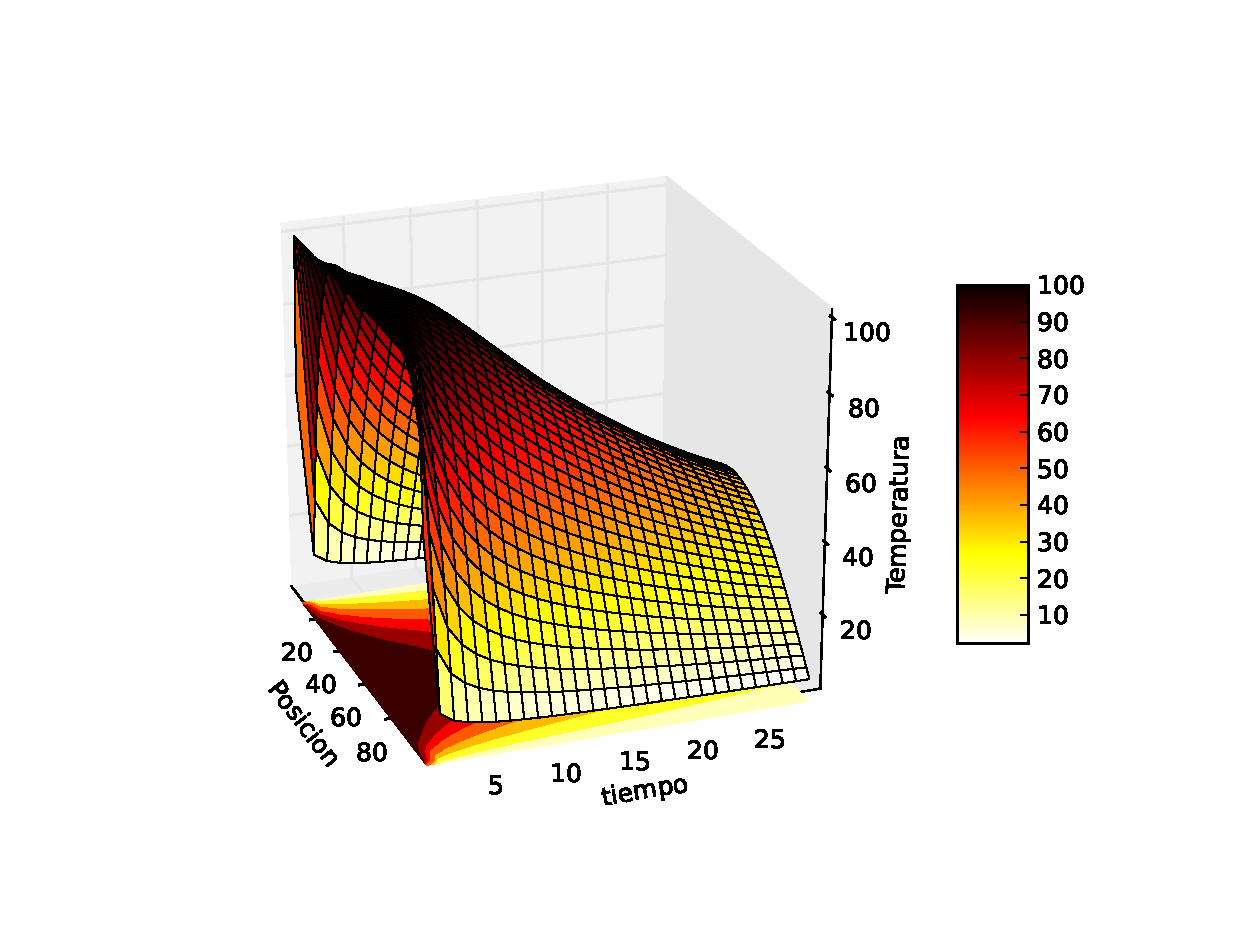
\includegraphics[scale=0.5]{EqCalor01.eps}  
\end{figure}
\end{frame}
\section{Problemas a resolver a cuenta de examen}
\begin{frame}
\frametitle{Problemas a resolver}
Se hacen algunos cambios en el planteamiento del problema, pero el algoritmo que hay que usar es el mismo, hay que resolver los siguientes casos:
\begin{enumerate}
\item Distribución inicial de temperatura de forma senoidal: $\sin( \pi x / L)$
\item Dos barras en contacto cada una con diferente temperatura.
\item Modificación de la ecuación de calor para incluir un término y obtener la ley de enfriamiento de Newton.
\end{enumerate}
\end{frame}
\subsection{Problema 1}
\begin{frame}
\frametitle{Problema 1}
Distribución inicial de temperatura de forma senoidal: $\sin( \pi x / L)$
\\
\bigskip
Utiliza las mismas constantes que en el primer ejemplo. Puedes comparar los resultados con la solución analítica:
\[ T(x,t) = \sin \left( \dfrac{\pi x}{L} \right) \exp(-\dfrac{\pi^{2}RT}{L^{2}}), \hspace{1cm} R=\dfrac{K}{C \rho} \]
\end{frame}
\begin{frame}
\frametitle{Solución del problema con la distribución de temperatura senoidal}
\begin{figure}
	\centering
	\includegraphics[scale=0.5]{Eqcalor04.eps}  
\end{figure}
\end{frame}
\begin{frame}
\frametitle{Problema con la distribución senoidal -rotada-}
\begin{figure}
	\centering
	\includegraphics[scale=0.5]{Eqcalor05.eps}  
\end{figure}
\end{frame}
\subsection{Problema 2}
\begin{frame}
\frametitle{Problema 2}
Dos barras en contacto cada una con diferente temperatura.
\\
\bigskip
Supongamos que tenemos dos barras idénticas, de 50 cm de longitud. Una de ellas se mantiene a $100^{\circ}$C y la otra a $50^{\circ}$C, se ponen en contacto a lo largo de su eje y los otros extremos se dejan a $0^{\circ}$C.
\\
\bigskip
Determina cómo varía la temperatura con respecto a la posición y al tiempo.
\end{frame}
\begin{frame}
\frametitle{Dos barras con diferente temperatura en contacto}
\begin{figure}
	\centering
	\includegraphics[scale=0.5]{Eqcalor06.eps}  
\end{figure}
\end{frame}
\begin{frame}
\frametitle{Dos barras en contacto -rotada-}
\begin{figure}
	\centering
	\includegraphics[scale=0.5]{Eqcalor07.eps}  
\end{figure}
\end{frame}
\subsection{Problema 3}
\begin{frame}
\frametitle{Problema 3}
Modificación de la ecuación de calor para incluir un término y obtener la ley de enfriamiento de Newton.
\\
\bigskip
Imagina ahora que la barra que estaba aislada (el problema con el que comenzamos la clase), se deja en contacto con el ambiente que se encuentra a una temperatura $T_{e}$, tal que es diferente a la temperatura inicial de la barra.
\\
\bigskip
La ley de enfriamiento de Newton nos dice que la razón de cambio de la temperatura debido a la radiación es:
\[ \dfrac{\partial T}{\partial t} = - h (T- T_{e}) \]
\end{frame}
\begin{frame}
La ecuación de calor se modifica, quedando:
\[ \dfrac{\partial T(x,t)}{\partial t} = \dfrac{K}{C \rho} \dfrac{\partial^{2}T}{\partial x^{2}} - h T(x,t)\]
Ajusta el algoritmo y el programa para introducir el término de enfriamiento de Newton a lo largo de la barra. Compara el enfriamiento de esta barra con el ejemplo de la barra aislada.
\end{frame}
\begin{frame}
\frametitle{Barra aislada}
\begin{figure}
	\centering
	\includegraphics[scale=0.5]{Eqcalor08.eps}  
\end{figure}
\end{frame}
\begin{frame}
\frametitle{Ley de enfriamiento de Newton, con $T_{e}=25^{\circ}C$}
\begin{figure}
	\centering
	\includegraphics[scale=0.5]{Eqcalor09.eps}  
\end{figure}
\end{frame}
\end{document}